\chapter{Introduction}
Crystallisation is one of the oldest forms of phase separation used by humanity\cite{Schoen1956}, put simply, it is the formation and growth 
of a new structured phase within a disordered bulk phase. This has 
applications in a number of industries such as pharmaceuticals, food 
production, and electronics \cite{Myerson2002}. Where the extraction 
of dilute materials can help improve product quality while keeping 
production costs low. The industrialisation of crystallisation has 
allowed engineers to reliably and efficiently induce the crystal 
formation within a bulk phase. However, while on a large scale 
crystallisation is seemingly an understood physical process, just a 
small amount of investigation into the literature reveals that at a 
micro scale there is yet to be unifying theory that can accurately 
explain the process of crystallisation \cite{Fu2021}. Of which there 
two primary areas of focus, nucleation and crystal growth. The latter 
focusing on how an already stable crystal grows and how it takes on its 
final shape. Whereas the former is more concerned with which factors 
contribute to its formation in order to control crystal growth.SW

In this chapter we will outline our current understanding of nucleation,
why there is a gap in the literature, and why there is still a need for
local control of nucleation events. Furthermore, we will also highlight
recent developments involving the use of optical tweezers (and other 
laser based methods) in order to develop our understanding of nucleation.
Lastly we highlight the connection between optical tweezer's ability to 
probe fluid viscosity via rotational motion, and the known link between
nucleation and fluid flow, to propose a novel potential method of 
creating localised nucleation events.
 
\section{Nucleation}
Nucleation is an example of a binary phase separation, where a dilute phase 
is miscible in a bulk phase, more often called the solute and solvent 
respectively. Because of thermodynamics, the two can only remain in 
equilibrium while below a specific concentration ($C_{eq}$) - below which 
the chemical potential $\mu$ for a miscible solution is greater than the 
potential required to separate the two phases. Once $C_{eq}$ is exceeded 
there is a chemical potential difference driving the solution to separate 
the two phases. Since different combinations of solute and solvent will 
have different equilibrium concentrations, researchers often instead measure 
the ratio between the solute and solvent by using 'supersaturation', one 
form of measuring supersaturation is shown below \cite{Mullin2001}:
\begin{align}
	\label{eq:supersaturation}
	S(T) = \frac{C_{sol}}{C_{eq}(T)}
\end{align}

Where $C_{sol}$ is just the solute concentration, and $C_{eq}(T)$is the 
equilibrium concentration at temperature $T$. While the solution remains 
supersaturated there is a chemical potential driving force for the solute 
to coalesce and separate from the solution as an ordered solid, the first 
formation of the crystal is referred to as the nucleus and understanding its 
formation of has been the focus of researchers for decades now. Typically, 
for an industrial crystallisation process the working principle is based on 
controlling and manipulating the supersaturation of the system. Of course 
nucleation events in a variety of different situations which each require 
their own classification. 

\subsection{Primary \& Secondary nucleation}
From an industrial perspective, the nucleation process can be broadly 
categorised into either primary of secondary nucleation. The former 
describes the formation of an initial nucleus within the bulk phase, 
absent of any external stimuli. Primary nucleation is therefore considered 
stochastic as there is no reliable means of predicting where a nucleus
may form, or how long it will take. The only reliable indicator being 
that higher supersaturations will result in faster nucleation rates. At 
a small scale one can estimate the nucleation rate by making repeated 
measurements of sample solutions and seeing how many have nucleated 
after a given time, giving us a Poisson probability distribution.
\begin{align}
	P(t) = 1 - exp\left[-JV(t-t_g)\right] = \frac{M^*(t)}{M}
\end{align}

Where $J$ is the nucleation rate, $t_g$ is the 'growth time', $V$ is 
the volume of the individual samples, and $M^*(t)$ \& $M$ are the number 
of nucleated samples and the total number of samples used respectively.
While this is useful for studying the effects of different parameters at 
a small scale, for industrial applications there are to many external 
factors for primary nucleation to be the only 

In contrast, secondary nucleation is the result of a initial 
seed crystal inducing further nucleation within the bulk solution
\cite{Botsaris1976}. The research of Secondary nucleation is 
fascinating for its own merits; is it speculated that the 
supersaturation barrier is non-existent \cite{Cashmore2022}, 
Furthermore control of secondary nucleation events are crucial 
for ensuring reliable industrial crystalliser performance, 
fig.~\ref{fig:secondary} depicts an attempt of classifying  
every possible mechanism that could lead to secondary nucleation.
\begin{figure}[h!]
	\centering
	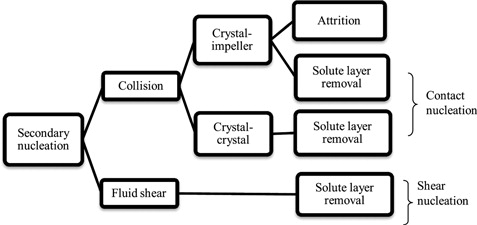
\includegraphics[width=0.95\linewidth]{secondary_nucleation.jpg}
	\caption{Secondary Nucleation mechanisms, classified by Agrawal 
		and Paterson \cite{Agrawal2015}}
	\label{fig:secondary}
\end{figure}

Its clear that preventing secondary nucleation is impossible
with so many possible mechanism, modelling its contribution
to the nucleation rate has been the area of research for some
time now \cite{Cashmore2022, Flannigan2023}. In most cases 
secondary nucleation is actually desirable for large scale 
production as primary nucleation is a stochastic process.

\section{Nucleation Theories}
A number of potential theories have been proposed to explain 
how nucleation occurs at a microscopic scale. In doing so 
we could potentially predict the expected yield of a given
crystalliser based on the initial conditions of the 
solution. Outlined below are some of the most popular theories
currently used to describe nucleation. 

\subsection{Classical Nucleation Theory (CNT)}
Sometimes referred to as 'Gibs Nucleation Theory' the original theory 
was first formed from the works of Volmer and Weber, and Frenkel 
\cite{Frenkel1939, Volmer1926}. While initially it was more focused 
into describing droplet formation in condensing vapours it was 
extrapolated to describe crystallisation. The central premise of 
classical theory is that nucleation occurs stochastically due to 
collisions between individual solute molecules, ions, or atoms. At the 
same time the bulk phase is resistant to the formation of a new phase. 
The competition between these random collisions and the bulk solution 
can be used to predict the probability of a newly formed nucleus.
 
Consider a supersaturated solution, after some time enough individual
sub units collide, forming a nucleus of volume $4\pi r^3/3$. The newly 
formed phase has a lower chemical potential than the surrounding solution, 
reducing the free energy of the system. Simultaneously, the formation of 
a new interface is resited by the bulk phase due to surface tension. 
The net free energy of the system for a nucleus of radius $r$ is given 
as \cite{Karthika2016}:
\begin{align}
	\Delta G = \frac{-4\pi r^3}{3v}k_BT\ln(S) + 4\pi r^{2}\sigma_{inf}
	\label{eq:CNT} 
\end{align}

Where $v$ is the approximate volume of an individual molecule, $k_B$ is 
the Boltzmann constant, and $\sigma_{inf}$ is the interfacial tension of 
the bulk solution. This assumes that the nucleus will have a spherical 
morphology so that the surface tension $\sigma_{inf}$ is a scalar value. 
Looking at \eqref{eq:CNT} suggests that there must be some critical size 
$r$ where the free energy gain from the nucleus exceeds the surface tension 
of the surrounding fluid. Plotting the free energy of the system against 
nucleus size reveals a critical size above which the gain in free energy 
exceeds the interfacial tension. Furthermore it shows how increasing the 
supersaturation of the system reduces said barrier. 
\begin{figure}[h!]
	\centering
	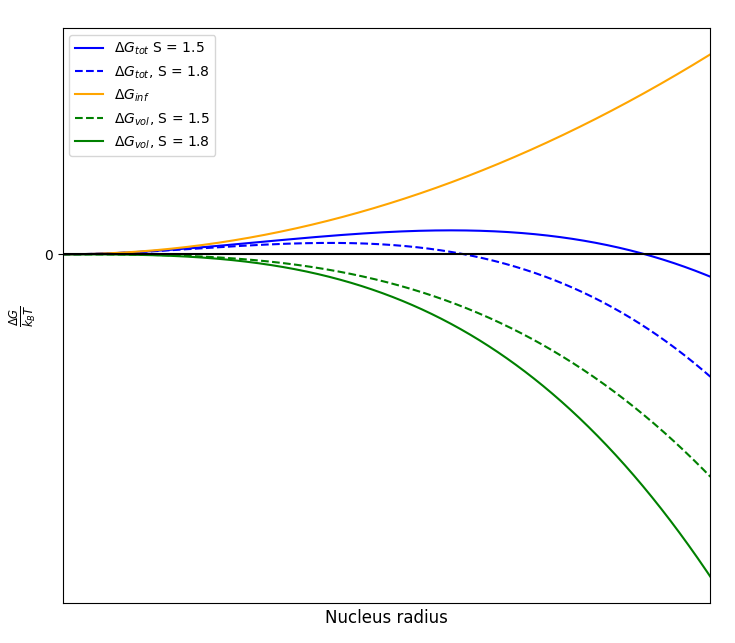
\includegraphics[width=\linewidth]{Free_Energy_Diagram.png}
	\caption{Free energy diagram of a newly formed nucleus according 
		     to the Classical Nucleation Theory. The total free energy (blue)
		     is due to the competition between the volume free energy gain
		     (green) and the interfacial free energy cost (orange). Dotted
		     lines are for a higher supersaturation than the solid lines,
		     the interfacial energy cost is independent of supersaturation.}
	\label{fig:free_energy}
\end{figure}

The maximum value of $\Delta G_{tot}$ is the free energy barrier that any 
newly formed nucleus needs to overcome in order to stabilise. The nucleation 
rate (the volume of new crystalline material formed per unit time), is 
therefore commonly defined as being dependent on the energy barrier $\Delta G^*$:
\begin{align}
	J = A \ exp \left[-\frac{\Delta G^*}{k_BT} \right]
\end{align}

Where $A$ is a pre-factor that can be fine tuned to the exact demands
of the system (typically involving Zeldovich Factor, $Z$) the free 
energy barrier can be found by finding the turning point of $\Delta G_{tot}$. 

CNT is often regarded as a good description of the macro system, its obvious
that for all crystallization systems there is an inherent energy barrier that 
dictates the nucleation rate. Where it falters is in its predictive ability, 
both in estimating nucleation rates \cite{Gharibeh2005, Vekilov2010}, and in 
the structure of newly formed nuclei \cite{Lee1999, Yau2001}. Recent studies 
suggest classical nucleation is merely one of many possible pathways that can 
be taken to produce a structured crystalline phase. Prompting the development of alternative theories to better describe the nucleation process.

\subsection{Two Step Nucleation}
The two step nucleation theory is an extension to the CNT that suggests 
that prior to nucleation, the solute will cluster together. This was 
shown via colloid simulations showed that short range (such as in proteins \cite{Wolde1997, Gliko2005}) interactions allow for the formation of a liquid-liquid metastable phase from which a new solid phase could form \cite{Anderson2002, Karthika2016}. Several papers later reported the 
presence of stable liquid-like clusters that formed prior to nucleation \cite{Savage2009, Wolde1997, Soga1999}. The formation of these clusters 
can be understood by Oswald's rule; which says that any crystallising 
system does not immediately take the path to the lowest possible energy 
state but instead first transitions to the state with the smallest free 
energy barrier \cite{Ostwald1897}. Further phase transitions can still 
occur but this pathway minimises the overall free energy cost. Initially 
it was suspected that the formation of the dense liquid phase was a 
result of stochastic density fluctuations in the system. However, 
simulations suggest that the the local bond order is a stronger driving 
force than the local density \cite{Tan2013}. Studies into two step 
nucleation in Glycine solutions have noted that the solutions need to be 
aged before the presence of clusters was detected. This suggests that 
there exist further barriers to the formation of clusters in some systems,
this has lead to instead calling this phenomena as Multi-step Nucleation.

\subsection{Non-classical Nucleation} 
The current research into two step nucleation (or now more commonly 
referred to as multi-step nucleation theory) is developing a robust 
framework to describe what nucleation pathway will occur given the 
initial conditions. Reviews of all currently documented nucleation 
pathways identified highlighted the fact the need for a the 
development of \textit{in situ} techniques that can induce nucleation 
locally but can also reliably identify the nucleation pathway across 
a broad range of experimental conditions \cite{Karthika2016, Fu2021}. 


%%%%%%%%%%%%%%%%%%%%%%%%%%%%%%%%%%%%%%%%%%%%%%%%%%%%%%%%%%%%%%%%%%%%%%%%%%%%%
%%%%%%%%%%%%%%%%%%%%%%%%%%%%%%%%%%%%%%%%%%%%%%%%%%%%%%%%%%%%%%%%%%%%%%%%%%%%%
\section{Crystallisation methods}
\subsection{Cooling Crystallisation}
For some binary mixtures the supersaturation is heavily dependent on 
the solution temperature, therefore a simple method of producing crystals 
is by cooling the mixture to induce crystal formation. At ambient 
temperatures the solute concentration is too high to be fully incorporated
into the solution ($S\gg 1$), after heating however the solute is fully 
dissolved into the solution ($S<1$). Now as the mixture is allowed to cool 
to room temperature the supersaturation will increase until crystal formation begins, the rate of cooling drastically influencing the size and number of crystals produced.

If $dT/dt$ is high then the final product will consist of large 
crystal and be low in number, as the nucleation rate is directly related
to the supersaturation only a handful of nuclei can form before the remaining
solute grows onto the surface. If $dT/dt$ is low then the final product will 
consist of smaller crystals and be far more numerous, as the supersaturation 
is so large that the new nuclei are forming continuously. Between these two 
extremes, one can define the meta-stable zone width, a region in the 
temperature-concentration phase space where both nucleation and crystal growth
can be reliably controlled. The lower limit being given by the solubility curve
of the binary mixture, and the upper limit being defined by the metastable zone.

\begin{figure}[h!]
	\includegraphics[width=\linewidth]{MSZW.png}
	\caption{Typical Concentration vs Temperature plot with the solubility curve (black) and metastable zone (red). 3 different cooling curves are shown as well: a high rate of cooling (orange) shows the mixture quickly dropping below the solubility curve resulting in no new nuclei forming; a low rate of cooling (green) shows the mixture exceeding the metastable zone, where now nucleation occurs freely; and a typical cooling rate (blue) shows how a typical cooling crystalliser will operate, sitting in the middle of the other two curves.}
	\label{fig:MSZW}
\end{figure}

The viability of cooling crystallisation is dependent on the meta-stable 
zone width, too narrow and the process is difficult to control, too wide 
and the crystal growth rate may be insufficient for the desired outcome.

\subsection{Evaporative Crystallisation}
In situations where control of the final product size or shape is not the main
focus, often the cheapest method of producing a crystalline product is simply
to allow the solvent evaporate and separate from the solute. Depending on the 
total volume of solvent to evaporate this process can take on time scale of 
several days to complete.

\subsection{Anti-solvent Crystallisation} 
Anti-solvent crystallisation is a more involved separation method ,
by adding a new solvent that is miscible with the old solvent but is 
immiscible with the solute, the solute's effective solubility is decreased.
As such, the solution becomes supersaturated. This has the trade off in that the overall mass ratio between the solvent and solute is now lower. Careful
measurement of the anti-solvent is required in order to ensure that the 
decrease in solubility is not out matched by the decrease in mass ratio.
Anti-solvent crystallisation is not as common due to the fact that not all
solutions will have an ideal anti-solvent candidate.

\section{Optical Tweezers}
\subsection{Background}
Optical tweezing has been a field of applied optics ever since the 1970s
when Ashkin \cite{Ashkin1970} first showed that focused light was capable 
of trapping micron sized particles due to light exerting 'radiation pressure'. 
The working principle was that a light source such as a laser could trap 
small objects within a 2D plane, as long as the light source had an 
approximately Gaussian profile. Soon after, Ashkin showed that the introduction 
of a microscope objective would allow one to focus the light source to a 
diffraction limited point that would stably trap small objects within a 
confined volume \cite{Ashkin1980}. This allowed Ashkin and others to study 
biological material and would later be used to probe microscopic properties 
such as the formation of colloidal aggregates \cite{Yi2021} to the drag 
forces exerted by a pure vacuum \cite{Ahn2018, Monteiro2018}. Due to the 
predictable behaviour of light, optical tweezers have become essential for 
measuring and exerting precise forces on the magnitude of pico-newtons 
allowing one to probe the material properties of the smallest materials. 

\subsection{Gaussian Beams}
A Gaussian Beam is a simplistic approximation of a laser beam, in 
short it is an unbounded plane wave whose intensity of the 
electromagnetic field falls off from the centre similar to a normal distribution. This is perfectly fine for beams with a divergence 
angle of $0^{\circ}$, but later studies into focused beams showed 
that the assumption of a Gaussian intensity profile is inaccurate. 
A study conducted by Lock and Gouesbet found that as the Gaussian 
beam was focused the fall off in the electric field would 
consequentially induce additional electromagnetic fields 
\cite{Lock1994}. As a result the shape of the beam profile diverges 
from a Gaussian profile for focused beams. Regardless, for optical 
trapping experiments it is useful to assume a near Gaussian beam as 
many descriptions of lasers are simply combinations of plane waves 
(with varying amplitudes and wave vectors).  More information on 
electromagnetic theory is covered in chapter 2 but for now any 
mention of a focused laser can be thought of as a Gaussian beam, 
unless specified otherwise. 

\subsection{Literature related to laser induced nucleation}
From as early as 1996 it has been known that laser irradiation is a viable
method of inducing nucleation within a supersaturated solution
\cite{Garetz1996}. The first reported case was notable as it used a 
1.064 $\mu m$ laser, the glycine solutions would appear transparent to
such a laser which would suggest there was no photo-chemical reaction.
Later studies into this phenomena found that the laser polarisation 
can influence the polymorph produced. With circularly polarised light 
producing $\alpha$-glycine and linearly polarised light forming
$\gamma$-glycine \cite{Garetz2002}. Future research has found nucleation 
can be induced by 1 of 3 routes.

\subsubsection{Non-Photochemical Laser Induced Nucleation}
Non-photochemical laser induced nucleation (NPLIN) involves irradiating 
a solution with a pulsed laser \cite{Garetz1996,Garetz2002,Sun2006}. 
The laser itself does not have to be heavily focused, instead irradiating
a large region of the solution all at once. The choice of laser is of
particular importance; with nucleation probability changing depending 
on the wavelength \cite{Kacker2017}. In addition, the choice of solute will 
effect the setup, not only because some solute's are unaffected, but also 
because there is a minimum laser threshold before nucleation is observed 
\cite{Garetz2002}. Several papers have debated the exact mechanism that 
induces NPLIN \cite{Garetz2002, Knott2011}. A suggested theory to this is 
an optical Kerr effect, for anisotropically charged solute molecules the 
electric field can reorient them to match the propagation direction 
\cite{Garetz2002}. If enough molecules are co-aligned the free energy 
barrier is reduced to allow for ambient nucleation \cite{Knott2011}. 
An alternative theory is the dielectric polarisation effect, in 
conditions that are unfavourable to cluster formation the polarising 
effect can stabilise the clusters \cite{Alexander2008}. As the cluster 
concentration rises so does the likelihood of nucleation \cite{Vekilov2010}. 
Both theories are similar to one another but where the optical Kerr theory
is limited to anisotropic solute molecules, the direct polarisation 
theory is more flexible. Regardless both theories struggle to explain
why the phenomena is not observed in all nucleation systems 
\cite{Korede2023}, such as acetamide which is similar to urea which 
does nucleate when irradiated \cite{Ward2016}. One of the benefits of 
NPLIN is that since the pulses are relatively low in their intensity 
they can be fired off quickly in succession, allowing for continuos 
crystallisation set ups. Overall, the NPLIN phenomena needs further 
research to properly describe its effects. The mean pulse intensity 
needs to be kept relatively low (on the order of $0.1-0.01 GW/cm^2$), 
as high intensity pulses lead to a completely different nucleation 
mechanism.


\subsubsection{High Intensity Laser Induced Nucleation}
High intensity laser induced nucleation (HILIN), where the pulse intensity 
is on the order of several $PW/cm^2$ is far simpler a mechanism to explain 
in comparison to NPLIN. The production of nuclei can be wholly associated 
to a cavitation process within the target solution, where the laser focus 
results in thermo-cavitation and the subsequent pressure wave leads to
a nucleation event around the focus of the laser \cite{Yoshikawa2005, 
Soare2011, Barber2019}. What remains in question is both how the physical 
properties (size, polymorph, etc) are influenced by the cavitation process, 
and how the pressure change triggers nucleation. The former has already 
been investigated; by adjusting the focal position Ikeda \textit{et al} 
could control the polymorph of indomethacin \cite{Ikeda2015}, this is not 
a universal method however, as it has also been shown that laser power can 
influence the crystal polymorph \cite{Wang2010}. The latter is a tricky 
task to address due to the fact that these cavitation bubbles form and 
collapse in less than $100\ \mu s$. Using fluorescence dyed proteins, 
researchers were able to observe a sudden spike in fluorescence just 
as the cavitation bubble began to collapse, they suggested that due 
to the collapse of the cavitation bubble the protein clusters are 
brought together at the lasers focal point. However, while the fluorescence 
imaging indicates a local concentration increase it is difficult to 
quantify this change depending on the size of the bubble \cite{Korede2023}. 
It has been suggested that in theory any solution can undergo HILIN 
\cite{Korede2023}, but proving such a theory requires a clear 
understanding of the phenomena both before and after cavitation occurs. 
Current research aims to combine experimental research with computer 
simulations to develop a universal theory, with the hope that this could 
also be related to NPLIN.   

\subsubsection{Trapping Induced Nucleation}
Lastly, there is trapping induced nucleation, this is where optical 
tweezers come into play. Due to the radiation pressure created by 
the focused beam, it is possible to manipulate the solute, this was 
demonstrated with amino acids such as glycine \cite{Tsuboi2009}. 
Whether or not a crystal forms is due to the location of the laser 
focus. When focusing on the cover slip, supersaturated solutions 
of glycine and $D_2O$ were shown to create a dense liquid droplet 
of glycine and water \cite{Yuyama2010, Yuyama2012}. The dipole 
moment of the glycine molecules is too small to be influenced by 
the optical trap, as such it would suggest that larger aggregates 
are being manipulated. Applying DLS analysis to the dense liquid 
region showed that it was populated by clusters that would 
consolidate together upon being focused by the optical trap 
\cite{Gowayed2021}. Molecular simulations of glycine solutions 
showed that these clusters are unstable when using pure glycine 
below the saturation point suggesting that the clusters are 
formed due to glycine reaction products \cite{Sweatman2022}. 
When the optical trap is moved from the cover slip to the 
air-solution interface, nucleation would occur before a dense 
liquid region could form \cite{Yuyama2010}. Repeated experiments 
where the laser is focused on the air-solution interface have 
lead to a variety of different nucleation events. In some 
instances the nucleation occurs spontaneously after a short 
period of time \cite{Yuyama2010}. Whereas allowing a solution to 
age results in the formation of amorphous precursors that when 
irradiated will nucleate immediately \cite{Liao2022}. The 
precursors are only seen when the solution is irradiated by an 
optical tweezer and the growth rate can be controlled somewhat 
by varying the laser power \cite{Liao2022}. The reason why 
nucleation is only seen at the air-solution interface is due 
to the limited molecular mobility close to the interface. 
Often tweezing experiments will use a hydrophilic coating to 
minimise the height of the solution droplet and further limit
the molecular mobility \cite{Yuyama2012, Gowayed2021}.

Walton and Wynne discussed a plausible model for how the tweezer 
focus could result in a nucleation event. Put simply, when the 
laser is focused at the solution the radiation pressure draws 
in solute material, creating a concentrated region of solute. 
This also creates a depleted region around the focus and raises 
the local temperature. When the laser is turned off the depleted 
region around the focus quickly cools back to the ambient 
temperature. This sudden cooling allows for nucleation to occur
just outside the focus.  

Laser induced nucleation has the potential to be a viable method 
for \textit{in-situ} studying of nucleation events. Using high 
numerical aperture lenses one can localise the nucleation event 
to a specific region of the solution. The current issue is that 
the mechanism behind laser induced nucleation is not fully 
understood, as such it is rather difficult to modify the laser 
for different solution parameters. Instead it may be more 
effective to manipulate the solution using trapped particles. 
An common method is by apply a torque to a trapped particle, 
creating a micro-rotor that can can generate fluid flow.

\subsection{Optical Torque}
It has long been known that electromagnetic fields can transfer linear and
angular momentum \cite{Beth1936MechanicalDA}; more accurately the field 
is said to have both orbital and spin momentum. Though there is some 
debate on how to decompose the total momentum into these two components 
\cite{Bruce2020, Svak2018}, for this project we do not need to calculate 
the exact quantities and will instead look at the broader effects of both 
components. Orbital angular momentum arises from the shape of the wavefront 
of the particular field in question; for simple Gaussian beams the wavefronts 
are uniform and equally spaced resulting in the typical radiation pressure 
that Ashkin and co demonstrated \cite{Ashkin1980}. However, higher order 
modes of a Gaussian beam (for example: Laguerre-Gaussian modes) have 
non-uniform wave fronts meaning the orbital momentum has both angular and
linear components; depending on the relative size of the target particle 
one can induce rotation, or orbiting \cite{Bruce2020, Courtial2000}. 

Spin angular momentum (SAM) is attributed to the spin density of the field, 
early research has shown that the spin density is non-zero for any beam despite
the fact that the total SAM transferred to a medium is 0 \cite{Svak2018, 
Bliokh2014}. This has sparked debate if SAM is even a physical quantity as 
it does not aid in the transport of energy directly \cite{Bliokh2014} and 
so cannot be directly observed in some cases despite being non-zero. This 
paradox is resolved by representing the wave as an array of spin momentum 
loops that all together cancel one-another out when the medium is homogeneous.
Spacial inhomogeneities cause these spin loops to no longer be equal, resulting
in non-zero spin density, anisotropic mediums (such as birefringent crystal 
lattices) experience a transfer of spin angular momentum, imparting an optical
torque.

Birefringence is a material property often seen in crystalline materials, 
if the crystal lattice has different refractive indices for varying 
polarisations of light. For circularly polarised light this inhomogeneity 
results in a high degree of SAM being transferred to the target object \cite{Parkin2009, Arita2016}, this has been exploited to rotate microspheres 
as fast as 1000 Hz while suspended in a bulk medium \cite{Arita2016} as well 
as a means of measuring the local temperature and shear response of said 
medium \cite{Millen2014, RodriguezSevilla2018}. Calculating the optical 
torque applied to a birefringent material is given via:
\begin{equation}
	\label{eq:opt_torque}
	\begin{aligned}
		\tau_{opt} =& -\frac{\epsilon}{2\omega_{laser}}E_0^2sin(kd(\Delta n))cos2\theta sin2\phi 
		\\ &+  \frac{\epsilon}{2\omega_{laser}}E_0^2 (1-cos(kd(\Delta n))sin2\phi)
	\end{aligned}
\end{equation}

Where $\theta$ is the angle between the particle's long axis and the 
polarisation vector of the local EM field, and $\phi$ is the phase shift 
in the EM field. The first term represents the 'orientational' torque which 
is due to the target particle being aligned with the EM amplitude, when 
aligned $\theta=0$ meaning the entire term is negligible for particle's with a stable orientation. For sphere's this is always the case as they lack a 
distinctive major axis. The second term is due purely to the polarisation 
of the optical trap, for circularly polarised light $\phi=\pi/4$ thus 
maximising the torque transferred to the target particle. Eq.~\eqref{eq:opt_torque} is only applicable for particles with a known
birefringence, but there are other mechanisms that result in optical torque.

A common example is shape induced birefringence. If a particle has an 
anisotropic shape, it is more susceptible to being polarised along its 
longer axis than its shorter axis. Consider, for example, an ellipsoid 
elongated along one of its primary axis' ($r_z > r_x = r_y$). In a 
plane polarised beam such a particle will align with the polarisation
vector. Therefore, the particle will rotate as angular momentum is 
transferred along its long axis. The common feature for shape induced
birefringence is that all of these particles are aligned in the plane
of polarisation. Often the optical torque experienced is far greater 
than similar spherical particles that are birefringent. Currently 
spherical dimers are being rotated in vacuums to measure quantum forces
and torques \cite{Ahn2018, Reimann2018}. There are some cases alternative 
cases where particles are rotated while not being aligned in the plane 
of the polarisation. However in these cases their shape is often 
specifically engineered to scatter light either clockwise or 
counter-clockwise \cite{Higurashi1994}. 

Other examples of optical torque is when an anisotropic particle is 
aligned with the beam's direction of propagation (in which case $\theta
=\pi/2$ and the first term disappears). This is analogous to an optically trapped sphere, where alongside a restoring force the particle also 
experiences a restoring torque. This seemingly random rotational motion
is referred to as libation \cite{Bruce2020}, often in typical suspension
trapping situations (where the particle is suspended in a fluid) the 
translational motion is washed out by the translational motion. As such, 
many experiments elect to trap in low pressure environments to precisely 
measure the optical torque being exerted by the optical trap \cite{Ahn2018}.
This has lead to experiments to try and achieve '0 kelvin' motion, where
by trapping a silica dimer they were able to restrict its motion using 
3 optical traps simultaneously. Despite this, they found that the dimer's
rotational motion about its long axis could not be controlled leading to
the undesired rotational modes \cite{Bang2020}.

The detection and measurement of optical torque is still a field of intense
research, not only does it have potential to understand quantum fluctuations
in a particle's motion but also allows for the creation of more effective
micro-rotors. The latter being especially pertinent for understanding the 
behaviour of fluids experiencing localised shearing.

\section{Shear induced Nucleation}
It has long been known that fluid shear rate plays a role in influencing
nucleation; however, the exact relationship between shear rate and nucleation
rate has only been recently understood for specific solutions. Theoretical research into shear induced nucleation suggests that there should be a 
slight increase in the nucleation rate at low shear rates, reaching a 
maximum increase in nucleation rate, and then at higher shear rates the 
nucleation rate begins to drop off. 

This has been shown theoretically for both simple colloidal \cite{Mura2016,
Debuysschere2023,Richard2015} and ice crystal formation \cite{Goswami2020}; however, no experimental work into these systems has been conducted to prove 
this is the case. There is some experimental evidence for this phenomena in 
simple salt and protein solutions - though the authors emphasise that mechanical agitation cannot be ruled out - there has not been a exhaustive study into the shearing effects apart from in glycine solutions. In \cite{Debuysschere2023} it was found that a shear rate of around $3000\ s^{-1}$ was the maximum shear rate that would yield the highest nucleation rate. Using the theoretical model established in \cite{Mura2016,2001} which modifies the CNT to account for the effects of a nucleus undergoing shearing, 
accounting for the fact that a nucleus' growth is undergoing competition 
between flow-mediated molecular transport and the strain applied by the 
flow field which inhibits the growth of the nucleus. There central 
conclusion (from both the theoretical and experimental results) is that 
there is an optimal shear rate in which the nucleation rate is maximised. 

However, a question that arises from this result, if there is a optimal 
shear rate in which molecular transport is maximised and strain is 
minimised, then surely there should also be a shear rate in which the 
molecular transport and strain are equal - allowing one to suspend a 
nucleus at a constant radius. In this scenario, the molecular transport 
would prevent the nucleus from dissolving, but the strain would prevent 
the nucleus from growing. This however would require one to be able 
to apply a continuous shear rate to a targeted nucleus with high precision, there is also no model for an individual nucleus in a continuous fluid 
field. 


\section{Significance of Thesis}
As I have hoped to make clear in the above introduction, the 
current state nucleation theory is rather cumbersome at a 
micro-level. Models such as CNT and multi-step nucleation are 
not sufficient for describing the myriad of potential pathways 
nucleation can go down. As suggested by some review articles, 
the best way to address this is by developing \textit{in-situ} 
methods that can study the pre nucleation phase in greater detail \cite{Fu2021}. Furthermore, the ability to localise nucleation 
allows for better characterisation of the kinetics of crystal 
growth. Laser induced nucleation stands to be an ideal method to 
study nucleation, as the laser output can be concentrated to a 
small area \cite{Korede2023}. This fine control over the local 
fluid would allow for individual nucleation events to be
characterised as a factor of the local fluid properties. One 
challenge lies in the fact that its clear that the local fluid 
properties have a direct influence on the likelihood of laser
induced nucleation from occurring \cite{Korede2023, Ward2016,
Yuyama2012, Liao2022}. 

A way around this would be to try and induce the local fluid 
without directly relying on the electromagnetic field. Optical 
tweezers can reliably do so already by applying an optical 
torque to a trapped particle in order to induce fluid flow 
\cite{Bishop2004, RobertsonAnderson2018}. It's already well
documented that shearing will enhance nucleation events at a
macro-level \cite{Debuysschere2023}. Micro-rheological studies 
using optical tweezing have been more interested in probing 
the local viscosity rather than try and use it as a means of 
shearing the fluid to induce crystal growth. 

\section{Overview}
Overall the aim of the PhD is to study viability of using 
micro-rotors to generate localised fluid flow around the 
beam focus. The results are reported in chapter 3, this is 
then succeeded by experimental work where we instead using 
a galvano-mirror to generate shear flow. While overall 
unsuccessful the addition of a moving beam focus showed 
that the growth of a nucleus can be localised around the 
trap focus. This presents a new insights for controlling
and studying the growth of a newly formed nucleus by 
precise movement of the trapping focus.

The latter chapters cover computer simulations into the 
behaviour of microscopic spherical dimers in an optical
trap. Prior research into dimers using back focal plane
interferometry has mostly considered their trapping 
behaviour to be similar to a single sphere but with a 
difference in trapping strength. Computer simulations
reveal a host of new behaviours dependent on the dimer's
size, orientation, proximity to the trapping focus, and 
even the polarisation of the trapping beam. The latter in
particular suggests that multi-spherical particles can act
as sophisticated micro-rotors. 

However, this raises a its own host of experimental challenges,
namely how do we characterise the behaviour of an arbitrary
particle. Relying on current characterisation techniques is not
possible as they are predicated on the trapping object to behave
like an isolated sphere. Two novel methods of measuring rotational 
motion are discussed in chapter 5; firstly via a novel detection 
fibre method that allows for instantaneous measurements of the 
orientational behaviour of optically trapped ellipsoids/dimers; 
and secondly we create a simulative quadrant photo diode that 
replicates laboratory results, utilising linear regression 
techniques we measure the change in orientation in order to 
measure the optical torque applied to a non-birefringent particle. 
